% Options for packages loaded elsewhere
\PassOptionsToPackage{unicode}{hyperref}
\PassOptionsToPackage{hyphens}{url}
%
\documentclass[
]{article}
\title{Preparing SCHISM-ICM netcdf files}
\author{Katie Lankowicz}
\date{19 April 2022}

\usepackage{amsmath,amssymb}
\usepackage{lmodern}
\usepackage{iftex}
\ifPDFTeX
  \usepackage[T1]{fontenc}
  \usepackage[utf8]{inputenc}
  \usepackage{textcomp} % provide euro and other symbols
\else % if luatex or xetex
  \usepackage{unicode-math}
  \defaultfontfeatures{Scale=MatchLowercase}
  \defaultfontfeatures[\rmfamily]{Ligatures=TeX,Scale=1}
  \setsansfont[]{Calibri}
\fi
% Use upquote if available, for straight quotes in verbatim environments
\IfFileExists{upquote.sty}{\usepackage{upquote}}{}
\IfFileExists{microtype.sty}{% use microtype if available
  \usepackage[]{microtype}
  \UseMicrotypeSet[protrusion]{basicmath} % disable protrusion for tt fonts
}{}
\makeatletter
\@ifundefined{KOMAClassName}{% if non-KOMA class
  \IfFileExists{parskip.sty}{%
    \usepackage{parskip}
  }{% else
    \setlength{\parindent}{0pt}
    \setlength{\parskip}{6pt plus 2pt minus 1pt}}
}{% if KOMA class
  \KOMAoptions{parskip=half}}
\makeatother
\usepackage{xcolor}
\IfFileExists{xurl.sty}{\usepackage{xurl}}{} % add URL line breaks if available
\IfFileExists{bookmark.sty}{\usepackage{bookmark}}{\usepackage{hyperref}}
\hypersetup{
  pdftitle={Preparing SCHISM-ICM netcdf files},
  pdfauthor={Katie Lankowicz},
  hidelinks,
  pdfcreator={LaTeX via pandoc}}
\urlstyle{same} % disable monospaced font for URLs
\usepackage[margin=1in]{geometry}
\usepackage{color}
\usepackage{fancyvrb}
\newcommand{\VerbBar}{|}
\newcommand{\VERB}{\Verb[commandchars=\\\{\}]}
\DefineVerbatimEnvironment{Highlighting}{Verbatim}{commandchars=\\\{\}}
% Add ',fontsize=\small' for more characters per line
\usepackage{framed}
\definecolor{shadecolor}{RGB}{248,248,248}
\newenvironment{Shaded}{\begin{snugshade}}{\end{snugshade}}
\newcommand{\AlertTok}[1]{\textcolor[rgb]{0.94,0.16,0.16}{#1}}
\newcommand{\AnnotationTok}[1]{\textcolor[rgb]{0.56,0.35,0.01}{\textbf{\textit{#1}}}}
\newcommand{\AttributeTok}[1]{\textcolor[rgb]{0.77,0.63,0.00}{#1}}
\newcommand{\BaseNTok}[1]{\textcolor[rgb]{0.00,0.00,0.81}{#1}}
\newcommand{\BuiltInTok}[1]{#1}
\newcommand{\CharTok}[1]{\textcolor[rgb]{0.31,0.60,0.02}{#1}}
\newcommand{\CommentTok}[1]{\textcolor[rgb]{0.56,0.35,0.01}{\textit{#1}}}
\newcommand{\CommentVarTok}[1]{\textcolor[rgb]{0.56,0.35,0.01}{\textbf{\textit{#1}}}}
\newcommand{\ConstantTok}[1]{\textcolor[rgb]{0.00,0.00,0.00}{#1}}
\newcommand{\ControlFlowTok}[1]{\textcolor[rgb]{0.13,0.29,0.53}{\textbf{#1}}}
\newcommand{\DataTypeTok}[1]{\textcolor[rgb]{0.13,0.29,0.53}{#1}}
\newcommand{\DecValTok}[1]{\textcolor[rgb]{0.00,0.00,0.81}{#1}}
\newcommand{\DocumentationTok}[1]{\textcolor[rgb]{0.56,0.35,0.01}{\textbf{\textit{#1}}}}
\newcommand{\ErrorTok}[1]{\textcolor[rgb]{0.64,0.00,0.00}{\textbf{#1}}}
\newcommand{\ExtensionTok}[1]{#1}
\newcommand{\FloatTok}[1]{\textcolor[rgb]{0.00,0.00,0.81}{#1}}
\newcommand{\FunctionTok}[1]{\textcolor[rgb]{0.00,0.00,0.00}{#1}}
\newcommand{\ImportTok}[1]{#1}
\newcommand{\InformationTok}[1]{\textcolor[rgb]{0.56,0.35,0.01}{\textbf{\textit{#1}}}}
\newcommand{\KeywordTok}[1]{\textcolor[rgb]{0.13,0.29,0.53}{\textbf{#1}}}
\newcommand{\NormalTok}[1]{#1}
\newcommand{\OperatorTok}[1]{\textcolor[rgb]{0.81,0.36,0.00}{\textbf{#1}}}
\newcommand{\OtherTok}[1]{\textcolor[rgb]{0.56,0.35,0.01}{#1}}
\newcommand{\PreprocessorTok}[1]{\textcolor[rgb]{0.56,0.35,0.01}{\textit{#1}}}
\newcommand{\RegionMarkerTok}[1]{#1}
\newcommand{\SpecialCharTok}[1]{\textcolor[rgb]{0.00,0.00,0.00}{#1}}
\newcommand{\SpecialStringTok}[1]{\textcolor[rgb]{0.31,0.60,0.02}{#1}}
\newcommand{\StringTok}[1]{\textcolor[rgb]{0.31,0.60,0.02}{#1}}
\newcommand{\VariableTok}[1]{\textcolor[rgb]{0.00,0.00,0.00}{#1}}
\newcommand{\VerbatimStringTok}[1]{\textcolor[rgb]{0.31,0.60,0.02}{#1}}
\newcommand{\WarningTok}[1]{\textcolor[rgb]{0.56,0.35,0.01}{\textbf{\textit{#1}}}}
\usepackage{graphicx}
\makeatletter
\def\maxwidth{\ifdim\Gin@nat@width>\linewidth\linewidth\else\Gin@nat@width\fi}
\def\maxheight{\ifdim\Gin@nat@height>\textheight\textheight\else\Gin@nat@height\fi}
\makeatother
% Scale images if necessary, so that they will not overflow the page
% margins by default, and it is still possible to overwrite the defaults
% using explicit options in \includegraphics[width, height, ...]{}
\setkeys{Gin}{width=\maxwidth,height=\maxheight,keepaspectratio}
% Set default figure placement to htbp
\makeatletter
\def\fps@figure{htbp}
\makeatother
\setlength{\emergencystretch}{3em} % prevent overfull lines
\providecommand{\tightlist}{%
  \setlength{\itemsep}{0pt}\setlength{\parskip}{0pt}}
\setcounter{secnumdepth}{-\maxdimen} % remove section numbering
\usepackage{setspace}\onehalfspacing
\usepackage{float}
\ifLuaTeX
  \usepackage{selnolig}  % disable illegal ligatures
\fi

\begin{document}
\maketitle

~~~~~~~Jeremy Testa and his model working group have provided me with
output from a Semi-implicit Cross-scale Hydroscience Integrated System
Model - Integrated Compartment Model. This is a three-dimensional
unstructured grid that simulates environmental variables in the Corsica
River in 2006. We will use these data to create dynamic environmental
conditions that will be used in an individual-based model (IBM) of
menhaden movement. Extensive pre-processing is needed before we can put
these data into our IBM, which we hope will closely resemble an
idealized shallow estuarine tidal tributary. This document will describe
the pre-processing methods used.

\hypertarget{original-grid-space}{%
\subsection{Original grid space}\label{original-grid-space}}

~~~~~~~The bounding box around the modeled portion of the Corsica is
approximately 7400m x 5600m. The Corsica is similar to St.~Leonard
Creek, which is our field data collection area-- the surrounding
watershed is not highly developed. It is mostly agricultural land or
forested buffers around lots. St.~Leonard Creek is mostly forested land
with some agricultural and residential area.\\
\hspace*{0.333em}\hspace*{0.333em}\hspace*{0.333em}\hspace*{0.333em}\hspace*{0.333em}\hspace*{0.333em}\hspace*{0.333em}Grid
cells in the model are triangles of varying shape and size. The cells
meet at nodes, and environmental variables are simulated through time at
these nodes. The high spatial resolution of the grid cells and high
temporal resolution of simulated environmental variables is a good match
for our proposed fine-scale IBM.

\singlespacing

\begin{figure}[H]
  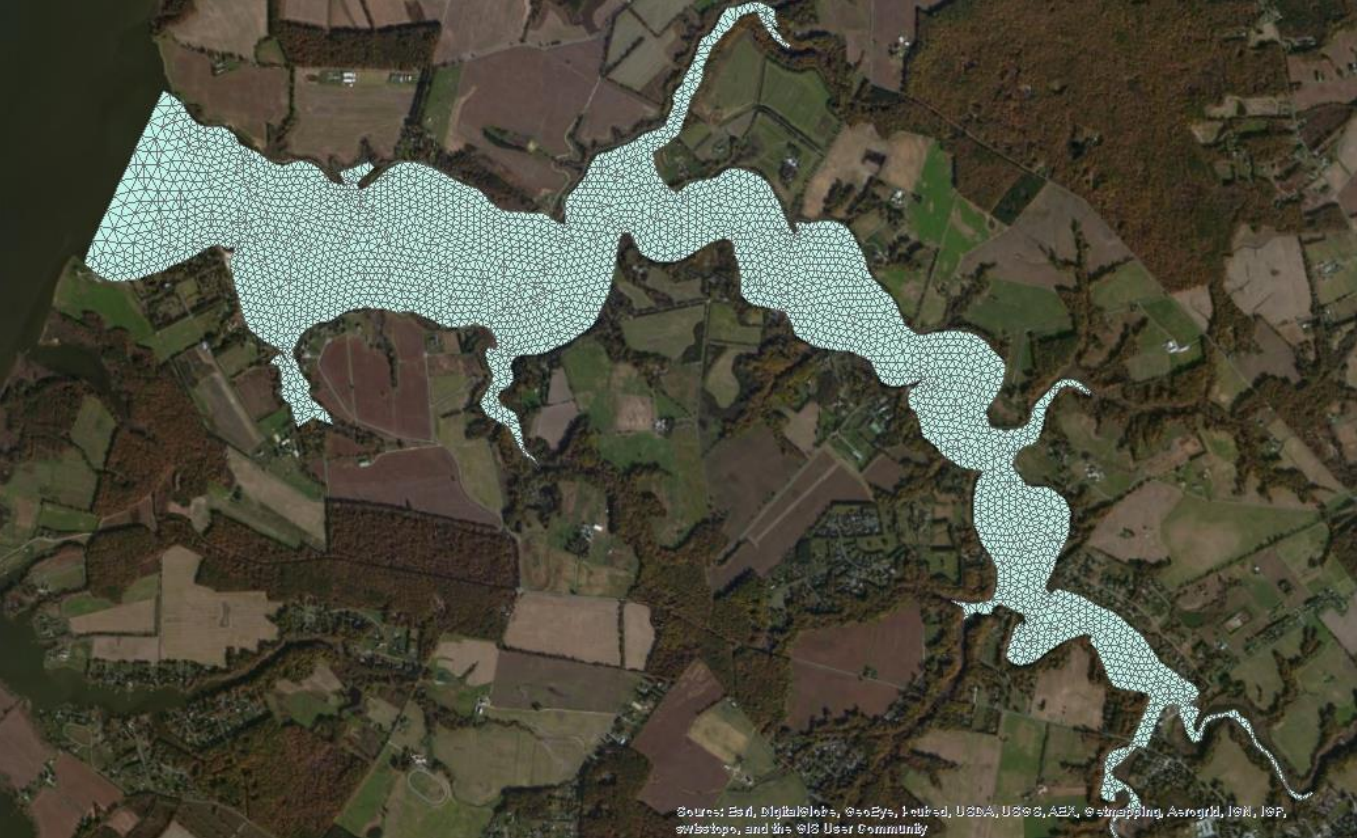
\includegraphics{Corsica_grid.png}
  \caption{Grid cells in the Corsica River}
\end{figure}

\begin{figure}[H]
  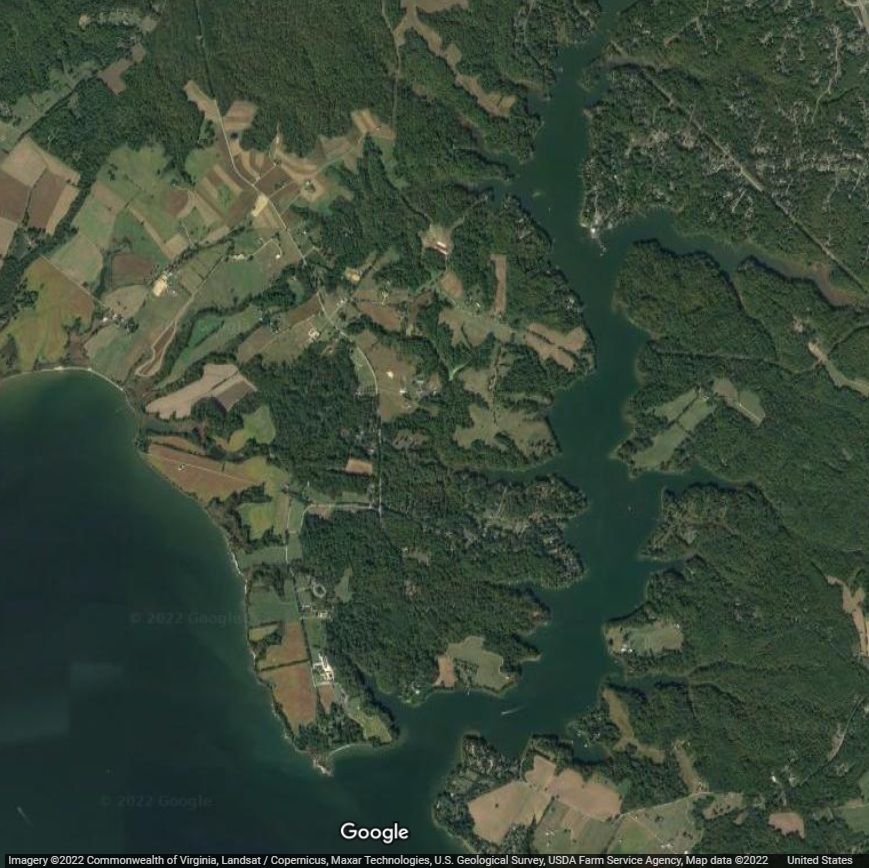
\includegraphics{StLeonardCreek.png}
  \caption{Land use surrounding St. Leonard Creek}
\end{figure}

\newpage
\onehalfspacing

\hypertarget{load-data}{%
\subsection{Load data}\label{load-data}}

~~~~~~~The first step is to open the \texttt{netcdf} file and view the
variables included.

\singlespacing

\begin{Shaded}
\begin{Highlighting}[]
\NormalTok{nc\_data }\OtherTok{\textless{}{-}} \FunctionTok{nc\_open}\NormalTok{(}\FunctionTok{paste0}\NormalTok{(}\StringTok{\textquotesingle{}C:/Users/klank/OneDrive/\textquotesingle{}}\NormalTok{,}
                          \StringTok{\textquotesingle{}Desktop/CBP\_Corsica\_SCHISM.nc\textquotesingle{}}\NormalTok{))}
\FunctionTok{names}\NormalTok{(nc\_data}\SpecialCharTok{$}\NormalTok{var)}
\end{Highlighting}
\end{Shaded}

\begin{verbatim}
##  [1] "ICM_21"              "ICM_3"               "ICM_4"              
##  [4] "ICM_5"               "ICM_6"               "ICM_7"              
##  [7] "ICM_Chl"             "SCHISM_hgrid_face_x" "SCHISM_hgrid_face_y"
## [10] "SCHISM_hgrid_node_x" "SCHISM_hgrid_node_y" "depth"              
## [13] "elev"                "salt"                "sigma_h_c"          
## [16] "sigma_theta_b"       "sigma_theta_f"       "temp"
\end{verbatim}

\onehalfspacing

~~~~~~~The horizontal space of the grid is reported in the xy
coordinates of the grid faces and grid nodes. There are 5029 grid cells
(and therefore grid face coordinate values) and 2888 grid nodes.\\
\hspace*{0.333em}\hspace*{0.333em}\hspace*{0.333em}\hspace*{0.333em}\hspace*{0.333em}\hspace*{0.333em}\hspace*{0.333em}Each
grid cell has a static \texttt{depth} value and a temporally dynamic
\texttt{elev} value. The value of \texttt{depth} is the base depth of
the water in that cell. The value of \texttt{elev} is water depth
fluctuation due to tides. To find the true depth of water at any xy
point at any time \emph{i}, we need to add the base depth of the cell
with the tidal flucation within the cell at time \emph{i}.\\
\hspace*{0.333em}\hspace*{0.333em}\hspace*{0.333em}\hspace*{0.333em}\hspace*{0.333em}\hspace*{0.333em}\hspace*{0.333em}The
grid also predicts environmental variables through the water column by
using sigma layers. These layers vary in thickness, but always cover the
entire water column from surface to the river bottom. We know from prior
data exploration and communication with the model's creators that the
Corsica only experiences episodic stratification. Therefore, we are not
overly concerned by the sigma layers that make up the vertical dimension
of the model and can simply pull the surface layer values. In the
future, we could consider using other sigma layers or averaging the
environmental conditions in a cell through all its sigma layers.\\
\hspace*{0.333em}\hspace*{0.333em}\hspace*{0.333em}\hspace*{0.333em}\hspace*{0.333em}\hspace*{0.333em}\hspace*{0.333em}Environmental
variables of interest are salinity, temperature, dissolved oxygen (here
called \texttt{ICM\_21}), and chlorophyll. All variables but chlorophyll
are simulated at the grid nodes. Chlorophyll is simulated at the grid
faces. This is because Chlorophyll is not a state variable, but rather a
property of phytoplankton biomass within the cell. We can alternatively
calculate the chlorophyll at every node by adding the biomass of all
phytoplankton variables (\texttt{ICM\_3}: Diatom, \texttt{ICM\_4}: Green
Algae, \texttt{ICM\_5}: Cyanobacteria) and multiplying them by 0.04,
which is the C:Chl ratio used by the model. We will compute chlorophyll
in this alternative way to match the xy grid the other environmental
variables are mapped to. This method was suggested by the model
creators.

\newpage

\hypertarget{subset-data}{%
\subsection{Subset data}\label{subset-data}}

\hypertarget{time}{%
\subsubsection{Time}\label{time}}

~~~~~~~We now need to start loading in our variables and paring them
down. We will start with time. The model simulates conditions in the
Corisca at an hour time step for the entire year of 2006, but we only
need the summer season. We have defined this time period as 1 June
through 31 August. Time in the model is recorded as seconds from an
origin point, which is 00:00:00 on 1 January 2006. We can convert to a
conventional timestamp, identify the seconds values of 00:00:00 1 June
2006 and 23:00:00 31 August 2006, and create a subsetting index from
these bounds.

\singlespacing

\begin{Shaded}
\begin{Highlighting}[]
\CommentTok{\# Load time variable}
\NormalTok{time }\OtherTok{\textless{}{-}} \FunctionTok{ncvar\_get}\NormalTok{(nc\_data, }\StringTok{"time"}\NormalTok{)}

\CommentTok{\# Create conventional timestamps}
\NormalTok{f }\OtherTok{\textless{}{-}} \FunctionTok{as.data.frame}\NormalTok{(time)}
\NormalTok{f}\SpecialCharTok{$}\NormalTok{timestamp }\OtherTok{\textless{}{-}}\NormalTok{ f}\SpecialCharTok{$}\NormalTok{time}\SpecialCharTok{/}\DecValTok{60}\SpecialCharTok{/}\DecValTok{60}\SpecialCharTok{/}\DecValTok{24}
\NormalTok{f}\SpecialCharTok{$}\NormalTok{timestamp }\OtherTok{\textless{}{-}} \FunctionTok{chron}\NormalTok{(f}\SpecialCharTok{$}\NormalTok{timestamp, }\AttributeTok{origin=}\FunctionTok{c}\NormalTok{(}\AttributeTok{month=}\DecValTok{1}\NormalTok{, }\AttributeTok{day=}\DecValTok{1}\NormalTok{, }\AttributeTok{year=}\DecValTok{2006}\NormalTok{))}
\NormalTok{f}\SpecialCharTok{$}\NormalTok{timestamp }\OtherTok{\textless{}{-}} \FunctionTok{as.Date}\NormalTok{(f}\SpecialCharTok{$}\NormalTok{timestamp)}

\CommentTok{\# Create vector of appropriate dates}
\NormalTok{dates }\OtherTok{\textless{}{-}} \FunctionTok{seq}\NormalTok{(}\FunctionTok{as.Date}\NormalTok{(}\StringTok{"2006{-}06{-}01"}\NormalTok{), }\FunctionTok{as.Date}\NormalTok{(}\StringTok{"2006{-}08{-}31"}\NormalTok{), }\AttributeTok{by=}\StringTok{\textquotesingle{}days\textquotesingle{}}\NormalTok{)}

\CommentTok{\# Subset f so only appropriate dates remain}
\NormalTok{f }\OtherTok{\textless{}{-}} \FunctionTok{subset}\NormalTok{(f, f}\SpecialCharTok{$}\NormalTok{timestamp }\SpecialCharTok{\%in\%}\NormalTok{ dates)}
\FunctionTok{row.names}\NormalTok{(f) }\OtherTok{\textless{}{-}} \ConstantTok{NULL}

\CommentTok{\# Pull minimum and maximum timestamps}
\NormalTok{mintime }\OtherTok{\textless{}{-}}\NormalTok{ f}\SpecialCharTok{$}\NormalTok{time[}\DecValTok{1}\NormalTok{]}
\NormalTok{maxtime }\OtherTok{\textless{}{-}}\NormalTok{ f}\SpecialCharTok{$}\NormalTok{time[}\FunctionTok{nrow}\NormalTok{(f)]}

\CommentTok{\# Create subsetting index by time}
\NormalTok{timidx }\OtherTok{\textless{}{-}} \FunctionTok{which}\NormalTok{(nc\_data}\SpecialCharTok{$}\NormalTok{dim}\SpecialCharTok{$}\NormalTok{time}\SpecialCharTok{$}\NormalTok{vals }\SpecialCharTok{\textgreater{}}\NormalTok{ mintime }\SpecialCharTok{\&}
\NormalTok{                nc\_data}\SpecialCharTok{$}\NormalTok{dim}\SpecialCharTok{$}\NormalTok{time}\SpecialCharTok{$}\NormalTok{vals }\SpecialCharTok{\textless{}}\NormalTok{ maxtime)}

\CommentTok{\# Convert to data frame}
\NormalTok{time }\OtherTok{\textless{}{-}} \FunctionTok{as.data.frame}\NormalTok{(time)}

\CommentTok{\# Create index of steps}
\NormalTok{time}\SpecialCharTok{$}\NormalTok{sidx }\OtherTok{\textless{}{-}} \FunctionTok{seq}\NormalTok{(}\DecValTok{1}\SpecialCharTok{:}\FunctionTok{nrow}\NormalTok{(time))}

\CommentTok{\# Subset so only times of interest are included}
\NormalTok{time }\OtherTok{\textless{}{-}}\NormalTok{ time[time}\SpecialCharTok{$}\NormalTok{sidx }\SpecialCharTok{\%in\%}\NormalTok{ timidx,]}

\CommentTok{\# Create new index of steps, with 1 being first included in model}
\NormalTok{time}\SpecialCharTok{$}\NormalTok{tidx }\OtherTok{\textless{}{-}} \FunctionTok{seq}\NormalTok{(}\DecValTok{1}\SpecialCharTok{:}\FunctionTok{nrow}\NormalTok{(time))}

\CommentTok{\# Add a more legible timestamp for later mapping purposes}
\NormalTok{time}\SpecialCharTok{$}\NormalTok{timestamp }\OtherTok{\textless{}{-}}\NormalTok{ time}\SpecialCharTok{$}\NormalTok{time}\SpecialCharTok{/}\DecValTok{60}\SpecialCharTok{/}\DecValTok{60}\SpecialCharTok{/}\DecValTok{24}
\NormalTok{time}\SpecialCharTok{$}\NormalTok{timestamp }\OtherTok{\textless{}{-}} \FunctionTok{chron}\NormalTok{(time}\SpecialCharTok{$}\NormalTok{timestamp, }
                        \AttributeTok{origin=}\FunctionTok{c}\NormalTok{(}\AttributeTok{month=}\DecValTok{1}\NormalTok{, }\AttributeTok{day=}\DecValTok{1}\NormalTok{, }\AttributeTok{year=}\DecValTok{2006}\NormalTok{))}

\CommentTok{\# Convert chron to POSIXct (add 3 hours, some kind of timezone issue)}
\NormalTok{time}\SpecialCharTok{$}\NormalTok{timestamp }\OtherTok{\textless{}{-}} \FunctionTok{as.POSIXct}\NormalTok{(time}\SpecialCharTok{$}\NormalTok{timestamp)}\SpecialCharTok{+} \FunctionTok{hours}\NormalTok{(}\DecValTok{3}\NormalTok{)}

\CommentTok{\# Remove intermediates}
\FunctionTok{rm}\NormalTok{(f, dates, mintime, maxtime)}
\end{Highlighting}
\end{Shaded}

\onehalfspacing

\hypertarget{horizontal-grid}{%
\subsubsection{Horizontal grid}\label{horizontal-grid}}

~~~~~~~Now we will load the horizontal grid nodes. We want to subset to
a portion of the total model to better match our idealized grid. The
idealized grid is meant to be a simple representation of the St.~Leonard
Creek transect, which is typically 2500m long and centered across 500m
of water. I have chosen a segment of the model that approximates those
proportions. This is the section between Emory Creek (the largest creek
on the North shore of the River, closer to mouth) and Alder Branch (the
next creek on the North shore moving upstream, closer to head). I will
manipulate the nodes in this segment to more closely fit in our
idealized rectangular model space.\\
\hspace*{0.333em}\hspace*{0.333em}\hspace*{0.333em}\hspace*{0.333em}\hspace*{0.333em}\hspace*{0.333em}\hspace*{0.333em}\hspace*{0.333em}\hspace*{0.333em}The
nodes here are not at all regularly spaced. That's part of the beauty of
the SCHISM setup-- it uses irregularly sized and shaped grid cells to
vary resolution as needed. The nodes are therefore irregularly placed.
The river itself is also not a simple shape, but has many curves and
bends. The grid is shaped by these shores. We want to set up our IBM in
a rectangular grid space, so we will need to manipulate the nodes to
better fit within our chosen extent and shape. The entire feature needs
to be rotated so the ``mouth'' end is at the lower limit of our y-axis
and the ``head'' is at the upper limit of our y-axis. Nodes within the
feature need to be moved to give better coverage within the rectangular
space. Because this is an idealized space, it is not critical that nodes
are exactly the same distance and bearing to each other in the IBM as
they are in SCHISM-ICM output. We simply want to make sure that we
preserve the cross-channel and down-creek trends.\\
\hspace*{0.333em}\hspace*{0.333em}\hspace*{0.333em}\hspace*{0.333em}\hspace*{0.333em}\hspace*{0.333em}\hspace*{0.333em}Moving
the nodes in space will change the original xy coordinates, and
therefore we need to have another method of relating the environmental
variables to their matching nodes in space. This was done by creating an
ID for each of the nodes that was preserved throughout the point
manipulation. Environmental variables simulated at point \(x_{q}\),
\(y_{q}\) were given the same ID as the grid node that was originally at
point \(x_{q}\), \(y_{q}\). Therefore, environmental variables were
still matched with their original nodes even after the nodes were moved
in space.\\
\hspace*{0.333em}\hspace*{0.333em}\hspace*{0.333em}\hspace*{0.333em}\hspace*{0.333em}\hspace*{0.333em}\hspace*{0.333em}The
manipulation of nodes was best done in ArcMap. I have read the
manipulated nodes in below.

\singlespacing

\begin{Shaded}
\begin{Highlighting}[]
\CommentTok{\# Load in manipulated points}
\NormalTok{gri }\OtherTok{\textless{}{-}} \FunctionTok{read.csv}\NormalTok{(}\FunctionTok{paste0}\NormalTok{(}\StringTok{\textquotesingle{}G:/My Drive/Documents\_Backup/Modeling/\textquotesingle{}}\NormalTok{,}
                           \StringTok{\textquotesingle{}GIS/SCHISM\_pts3.csv\textquotesingle{}}\NormalTok{))}

\CommentTok{\# Create index of points to keep}
\NormalTok{keep\_pts }\OtherTok{\textless{}{-}}\NormalTok{ gri}\SpecialCharTok{$}\NormalTok{idx}
\CommentTok{\# Plot, maintain 1:1 aspect ratio}
\FunctionTok{plot}\NormalTok{(gri}\SpecialCharTok{$}\NormalTok{lon, gri}\SpecialCharTok{$}\NormalTok{lat, }\AttributeTok{asp=}\DecValTok{1}\NormalTok{, }\AttributeTok{xlab=}\StringTok{\textquotesingle{}Longitude (m)\textquotesingle{}}\NormalTok{, }\AttributeTok{ylab=}\StringTok{\textquotesingle{}Latitude (m)\textquotesingle{}}\NormalTok{,}
     \AttributeTok{pch=}\DecValTok{19}\NormalTok{, }\AttributeTok{cex=}\FloatTok{0.5}\NormalTok{)}
\end{Highlighting}
\end{Shaded}

\begin{figure}[H]
\includegraphics{work_with_ncdf_files/figure-latex/unnamed-chunk-3-1} \caption{Manipulated grid node positions}\label{fig:unnamed-chunk-3}
\end{figure}

\onehalfspacing

\hypertarget{depth-and-tidal-information}{%
\subsubsection{Depth and tidal
information}\label{depth-and-tidal-information}}

~~~~~~~Now we have an index of space-time locations that we are
interested in. We will pull the static base depth and dynamic tidal
fluctuations using these indexes.

\singlespacing

\begin{Shaded}
\begin{Highlighting}[]
\CommentTok{\# Read tidal info}
\NormalTok{ele }\OtherTok{\textless{}{-}} \FunctionTok{ncvar\_get}\NormalTok{(nc\_data, }\StringTok{"elev"}\NormalTok{)}

\CommentTok{\# Convert to dataframe}
\NormalTok{ele }\OtherTok{\textless{}{-}} \FunctionTok{as.data.frame}\NormalTok{(ele)}

\CommentTok{\# Subset to times of interest: removes columns for other times}
\NormalTok{ele }\OtherTok{\textless{}{-}}\NormalTok{ ele[,timidx]}

\CommentTok{\# Create location index (still have all locations)}
\NormalTok{ele}\SpecialCharTok{$}\NormalTok{idx }\OtherTok{\textless{}{-}} \FunctionTok{seq}\NormalTok{(}\DecValTok{1}\SpecialCharTok{:}\FunctionTok{nrow}\NormalTok{(ele))}

\CommentTok{\# Subset location index to only include points of interest}
\NormalTok{ele }\OtherTok{\textless{}{-}}\NormalTok{ ele[ele}\SpecialCharTok{$}\NormalTok{idx }\SpecialCharTok{\%in\%}\NormalTok{ keep\_pts,]}
\end{Highlighting}
\end{Shaded}

\newpage
\onehalfspacing

\hypertarget{environmental-variables}{%
\subsubsection{Environmental variables}\label{environmental-variables}}

~~~~~~~Next, we'll read in the other environmental variables. These will
be subset to only include the locations and times that we are interested
in. They will also only include the surface measurements-- sigma layer
5.\\
\hspace*{0.333em}\hspace*{0.333em}\hspace*{0.333em}\hspace*{0.333em}\hspace*{0.333em}\hspace*{0.333em}\hspace*{0.333em}The
chlorophyll variable will need to be calculated by summing the
phytoplankton inputs at each node and multiplying by the C:Chl ratio.\\
\hspace*{0.333em}\hspace*{0.333em}\hspace*{0.333em}\hspace*{0.333em}\hspace*{0.333em}\hspace*{0.333em}\hspace*{0.333em}We
will also calculate the true depth of water in space-time by adding the
static base depth with the dynamic changes in elevation due to tides.

\singlespacing

\begin{Shaded}
\begin{Highlighting}[]
\CommentTok{\# Identify variables of interest}
\NormalTok{data }\OtherTok{\textless{}{-}} \FunctionTok{c}\NormalTok{(}\StringTok{\textquotesingle{}salt\textquotesingle{}}\NormalTok{, }\StringTok{\textquotesingle{}temp\textquotesingle{}}\NormalTok{, }\StringTok{\textquotesingle{}ICM\_21\textquotesingle{}}\NormalTok{, }\StringTok{\textquotesingle{}ICM\_3\textquotesingle{}}\NormalTok{, }\StringTok{\textquotesingle{}ICM\_4\textquotesingle{}}\NormalTok{, }\StringTok{\textquotesingle{}ICM\_5\textquotesingle{}}\NormalTok{)}

\CommentTok{\# Loop to read in environmental variables}
\ControlFlowTok{for}\NormalTok{(i }\ControlFlowTok{in} \DecValTok{1}\SpecialCharTok{:}\FunctionTok{length}\NormalTok{(data))\{}
  \CommentTok{\# Read in variable}
\NormalTok{  varo }\OtherTok{\textless{}{-}} \FunctionTok{ncvar\_get}\NormalTok{(nc\_data, }\FunctionTok{paste0}\NormalTok{(data[i]))[}\DecValTok{5}\NormalTok{,,]}
  \CommentTok{\# Convert to dataframe}
\NormalTok{  varo }\OtherTok{\textless{}{-}} \FunctionTok{as.data.frame}\NormalTok{(varo)}
  \CommentTok{\# Subset to times of interest: removes columns for other times}
\NormalTok{  varo }\OtherTok{\textless{}{-}}\NormalTok{ varo[,timidx]}
  \CommentTok{\# Create location index (still have all locations)}
\NormalTok{  varo}\SpecialCharTok{$}\NormalTok{idx }\OtherTok{\textless{}{-}} \FunctionTok{seq}\NormalTok{(}\DecValTok{1}\SpecialCharTok{:}\FunctionTok{nrow}\NormalTok{(varo))}
  \CommentTok{\# Subset location index to only include points of interest}
\NormalTok{  varo }\OtherTok{\textless{}{-}}\NormalTok{ varo[varo}\SpecialCharTok{$}\NormalTok{idx }\SpecialCharTok{\%in\%}\NormalTok{ keep\_pts,]}
  \CommentTok{\# Identify variable name}
\NormalTok{  char }\OtherTok{\textless{}{-}} \FunctionTok{paste0}\NormalTok{(data[i])}
  \CommentTok{\# Rename variable to variable name}
\NormalTok{  varo }\OtherTok{\textless{}{-}} \FunctionTok{assign}\NormalTok{(char, varo)}
  \CommentTok{\# Remove intermediates}
  \FunctionTok{rm}\NormalTok{(varo, char)}
\NormalTok{\}}

\CommentTok{\# Calculate chlorophyll}
\CommentTok{\# Create duplicates of phytoplankton variables without index}
\NormalTok{ICM\_32 }\OtherTok{\textless{}{-}}\NormalTok{ ICM\_3}
\NormalTok{ICM\_32}\SpecialCharTok{$}\NormalTok{idx }\OtherTok{\textless{}{-}} \ConstantTok{NULL}
\NormalTok{ICM\_42 }\OtherTok{\textless{}{-}}\NormalTok{ ICM\_4}
\NormalTok{ICM\_42}\SpecialCharTok{$}\NormalTok{idx }\OtherTok{\textless{}{-}} \ConstantTok{NULL}
\NormalTok{ICM\_52 }\OtherTok{\textless{}{-}}\NormalTok{ ICM\_5}
\NormalTok{ICM\_52}\SpecialCharTok{$}\NormalTok{idx }\OtherTok{\textless{}{-}} \ConstantTok{NULL}

\CommentTok{\# Combine data for all phytoplankton variables}
\NormalTok{chl  }\OtherTok{\textless{}{-}} \FunctionTok{cbind}\NormalTok{(ICM\_32, ICM\_42, ICM\_52)}
\CommentTok{\# Add columns with matching names across all dataframes}
\NormalTok{chl }\OtherTok{\textless{}{-}} \FunctionTok{t}\NormalTok{(}\FunctionTok{rowsum}\NormalTok{(}\FunctionTok{t}\NormalTok{(chl), }\AttributeTok{group=}\FunctionTok{colnames}\NormalTok{(chl), }\AttributeTok{na.rm=}\NormalTok{T))}
\CommentTok{\# Convert to dataframe}
\NormalTok{chl }\OtherTok{\textless{}{-}} \FunctionTok{as.data.frame}\NormalTok{(chl)}
\CommentTok{\# Divide by C:Chl ratio (0.04)}
\NormalTok{chl }\OtherTok{\textless{}{-}}\NormalTok{ chl }\SpecialCharTok{/} \FloatTok{0.04}
\CommentTok{\# Copy over preserved index variable}
\NormalTok{chl}\SpecialCharTok{$}\NormalTok{idx }\OtherTok{\textless{}{-}}\NormalTok{ ICM\_3}\SpecialCharTok{$}\NormalTok{idx}
\CommentTok{\# Move index variable to last column}
\NormalTok{chl }\OtherTok{\textless{}{-}}\NormalTok{ chl }\SpecialCharTok{\%\textgreater{}\%}\NormalTok{ dplyr}\SpecialCharTok{::}\FunctionTok{select}\NormalTok{(}\SpecialCharTok{{-}}\NormalTok{idx, idx)}

\CommentTok{\# Rename dataframes to desired variable names}
\NormalTok{sal }\OtherTok{\textless{}{-}}\NormalTok{ salt}
\NormalTok{dox }\OtherTok{\textless{}{-}}\NormalTok{ ICM\_21}
\NormalTok{tem }\OtherTok{\textless{}{-}}\NormalTok{ temp}

\CommentTok{\# Calculate true depth {-}{-} depth plus elevation}
\CommentTok{\# Create duplicate of elevation without index}
\NormalTok{tdep }\OtherTok{\textless{}{-}}\NormalTok{ ele}
\NormalTok{tdep}\SpecialCharTok{$}\NormalTok{idx }\OtherTok{\textless{}{-}} \ConstantTok{NULL}
\CommentTok{\# Add depth }
\ControlFlowTok{for}\NormalTok{(i }\ControlFlowTok{in} \DecValTok{1}\SpecialCharTok{:}\FunctionTok{ncol}\NormalTok{(tdep))\{}
\NormalTok{  tdep[,i] }\OtherTok{\textless{}{-}}\NormalTok{ tdep[,i] }\SpecialCharTok{+}\NormalTok{ gri}\SpecialCharTok{$}\NormalTok{dep}
\NormalTok{\}}
\NormalTok{tdep}\SpecialCharTok{$}\NormalTok{idx }\OtherTok{\textless{}{-}}\NormalTok{ ele}\SpecialCharTok{$}\NormalTok{idx}

\CommentTok{\# Close netcdf file}
\FunctionTok{nc\_close}\NormalTok{(nc\_data)}

\CommentTok{\# Remove intermediates}
\FunctionTok{rm}\NormalTok{(ICM\_21, ICM\_3, ICM\_4, ICM\_5, }
\NormalTok{   ICM\_32, ICM\_42, ICM\_52,}
\NormalTok{   salt, temp, ele,}
\NormalTok{   nc\_data, keep\_pts, timidx, i, data)}
\end{Highlighting}
\end{Shaded}

\onehalfspacing

\hypertarget{checking}{%
\subsection{Checking}\label{checking}}

~~~~~~~All variables should have the same dimensions. There are 624
nodes of interest, 1 sigma layer of interest, and 2206 time steps of
interest. Let's check that we have the correct dimensions. Variables in
both space and time (eg. salt) will have an extra column: the index
variable we will keep to preserve mapping ability.

\singlespacing

\begin{Shaded}
\begin{Highlighting}[]
\FunctionTok{dim}\NormalTok{(time)}
\end{Highlighting}
\end{Shaded}

\begin{verbatim}
## [1] 2206    4
\end{verbatim}

\begin{Shaded}
\begin{Highlighting}[]
\FunctionTok{dim}\NormalTok{(gri)}
\end{Highlighting}
\end{Shaded}

\begin{verbatim}
## [1] 624   4
\end{verbatim}

\begin{Shaded}
\begin{Highlighting}[]
\FunctionTok{dim}\NormalTok{(sal);}\FunctionTok{dim}\NormalTok{(tem);}\FunctionTok{dim}\NormalTok{(dox);}\FunctionTok{dim}\NormalTok{(chl); }\FunctionTok{dim}\NormalTok{(tdep)}
\end{Highlighting}
\end{Shaded}

\begin{verbatim}
## [1]  624 2207
\end{verbatim}

\begin{verbatim}
## [1]  624 2207
\end{verbatim}

\begin{verbatim}
## [1]  624 2207
\end{verbatim}

\begin{verbatim}
## [1]  624 2207
\end{verbatim}

\begin{verbatim}
## [1]  624 2207
\end{verbatim}

\onehalfspacing

\hypertarget{combine}{%
\subsection{Combine}\label{combine}}

~~~~~~~We already have a dataframe of the node positions and static base
depth at those positions. This defines the grid space we will use. We
want to make sure that we keep things together, so we will combine all
environmental variables into a list. Time will remain a separate
dataframe.

\singlespacing

\begin{Shaded}
\begin{Highlighting}[]
\CommentTok{\# Gather environmental variables into list}
\NormalTok{env }\OtherTok{\textless{}{-}} \FunctionTok{list}\NormalTok{(sal, tem, dox, chl, tdep)}

\CommentTok{\# Name list items}
\FunctionTok{names}\NormalTok{(env) }\OtherTok{\textless{}{-}} \FunctionTok{c}\NormalTok{(}\StringTok{\textquotesingle{}sal\textquotesingle{}}\NormalTok{, }\StringTok{\textquotesingle{}tem\textquotesingle{}}\NormalTok{, }\StringTok{\textquotesingle{}dox\textquotesingle{}}\NormalTok{, }\StringTok{\textquotesingle{}chl\textquotesingle{}}\NormalTok{, }\StringTok{\textquotesingle{}tdep\textquotesingle{}}\NormalTok{)}

\CommentTok{\# Remove intermediates}
\FunctionTok{rm}\NormalTok{(sal, tem, dox, chl, tdep)}
\end{Highlighting}
\end{Shaded}

\onehalfspacing

\hypertarget{creation-of-model-space-raster}{%
\subsection{Creation of model space
raster}\label{creation-of-model-space-raster}}

~~~~~~~Next we'll make a blank raster of the desired proportions. We
want a 2500m by 500m grid. Desired grid cell resolution is 10m by 10m.
This translates to a grid that is 250 cells long and 50 cells wide.

\singlespacing

\begin{Shaded}
\begin{Highlighting}[]
\CommentTok{\# Set number of rows and columns}
\NormalTok{n.row }\OtherTok{\textless{}{-}} \DecValTok{250}\NormalTok{; n.col }\OtherTok{\textless{}{-}} \DecValTok{50}

\CommentTok{\# Create matrix of desired dimensions, rasterize}
\NormalTok{r }\OtherTok{\textless{}{-}} \FunctionTok{raster}\NormalTok{(}\FunctionTok{matrix}\NormalTok{(}\DecValTok{0}\NormalTok{, n.row, n.col))}

\CommentTok{\# Set extent to match points retained from SCHISM manipulation}
\CommentTok{\# Make sure extent is exactly 2500m by 500m so cell resolution is 10m}
\FunctionTok{extent}\NormalTok{(r) }\OtherTok{\textless{}{-}} \FunctionTok{c}\NormalTok{(}\FloatTok{403575.9}\NormalTok{, }\FloatTok{404075.9}\NormalTok{,}
               \DecValTok{4326232}\NormalTok{ , }\DecValTok{4328732}\NormalTok{  )}

\CommentTok{\# Set projection}
\CommentTok{\# NAD83 HARN StatePlane Maryland FIPS 1900 (m)}
\NormalTok{r}\SpecialCharTok{@}\NormalTok{crs }\OtherTok{\textless{}{-}} \FunctionTok{CRS}\NormalTok{(}\StringTok{"ESRI:102285"}\NormalTok{)}
\end{Highlighting}
\end{Shaded}

\newpage
\onehalfspacing

\hypertarget{test-of-raster-by-plotting-depth}{%
\subsubsection{Test of raster by plotting
depth}\label{test-of-raster-by-plotting-depth}}

~~~~~~~We'll test the success of our raster by plotting the static base
depth. Base depth at each cell will be interpolated using inverse
distance weighting interpolation. The four closest neighbors by
Euclidean distance will be considered. The inverse distance power needed
to complete IDP will be estimated using k-fold cross-validation methods.
K chosen for this interpolation is 10. Sample size is the number of
points, which is 624.

\singlespacing

\begin{Shaded}
\begin{Highlighting}[]
\CommentTok{\# Convert raster to SpatialPixels}
\NormalTok{rpix }\OtherTok{\textless{}{-}} \FunctionTok{as}\NormalTok{(r, }\StringTok{"SpatialPixels"}\NormalTok{)}

\CommentTok{\# Points to spatial points data frame}
\NormalTok{spdat }\OtherTok{\textless{}{-}}\NormalTok{ sp}\SpecialCharTok{::}\FunctionTok{SpatialPointsDataFrame}\NormalTok{(}
  \CommentTok{\# Coordinates set to lon and lat (will be same for all timesteps)}
  \AttributeTok{coords=}\NormalTok{gri[,}\FunctionTok{c}\NormalTok{(}\StringTok{"lon"}\NormalTok{, }\StringTok{"lat"}\NormalTok{)],}
  \CommentTok{\# Data set to variable at timestep i}
  \AttributeTok{data  =}\NormalTok{gri[,}\FunctionTok{c}\NormalTok{(}\StringTok{\textquotesingle{}idx\textquotesingle{}}\NormalTok{, }\StringTok{\textquotesingle{}dep\textquotesingle{}}\NormalTok{)],}
  \CommentTok{\# CRS set to NAD83 HARN StatePlane Maryland FIPS 1900 (m)}
  \AttributeTok{proj4string =} \FunctionTok{CRS}\NormalTok{(}\StringTok{"ESRI:102285"}\NormalTok{)}
\NormalTok{)}
\CommentTok{\# Rename dep to value, artifact of intamap package}
\FunctionTok{names}\NormalTok{(spdat}\SpecialCharTok{@}\NormalTok{data) }\OtherTok{\textless{}{-}} \FunctionTok{c}\NormalTok{(}\StringTok{\textquotesingle{}idx\textquotesingle{}}\NormalTok{, }\StringTok{\textquotesingle{}value\textquotesingle{}}\NormalTok{)}

\CommentTok{\# Suppress warning associated with CRS comments}
\FunctionTok{options}\NormalTok{(}\AttributeTok{warn=}\SpecialCharTok{{-}}\DecValTok{1}\NormalTok{)}

\CommentTok{\# Set up idwObject}
\NormalTok{idwObject }\OtherTok{\textless{}{-}}  \FunctionTok{createIntamapObject}\NormalTok{(}
  \CommentTok{\# Set observations to SpatialPointsDataFrame}
  \AttributeTok{observations        =}\NormalTok{ spdat,}
  \CommentTok{\# Set formula to universal kriging}
  \AttributeTok{formulaString       =} \FunctionTok{as.formula}\NormalTok{(value}\SpecialCharTok{\textasciitilde{}}\DecValTok{1}\NormalTok{),}
  \CommentTok{\# Set prediction locations to blank raster of model space}
  \AttributeTok{predictionLocations =}\NormalTok{ rpix,}
  \CommentTok{\# Set method to inverse distance weighting}
  \AttributeTok{class               =} \StringTok{"idw"}
\NormalTok{)}

\CommentTok{\# k{-}fold brute{-}force Cross{-}validation selection of IDP}
\CommentTok{\# Set k, typically 5 or 10}
\NormalTok{k }\OtherTok{\textless{}{-}} \DecValTok{10}
\CommentTok{\# Estimate best IDP for IDW interpolation}
\NormalTok{idwObject }\OtherTok{\textless{}{-}}  \FunctionTok{estimateParameters}\NormalTok{(}
\NormalTok{  idwObject,}
\CommentTok{\# Set range of possible inverse distance power values}
\CommentTok{\# min=0, max=5, step=0.05. All steps will be evaluated.}
  \AttributeTok{idpRange =} \FunctionTok{seq}\NormalTok{(}\FloatTok{0.00}\NormalTok{,}\FloatTok{5.00}\NormalTok{,}\FloatTok{0.05}\NormalTok{),}
\CommentTok{\# Call k{-}fold value}
  \AttributeTok{nfold=}\NormalTok{k}
\NormalTok{)}

\CommentTok{\# Interpolate using IDP chosen above}
\NormalTok{fitmax }\OtherTok{\textless{}{-}}\NormalTok{ gstat}\SpecialCharTok{::}\FunctionTok{gstat}\NormalTok{(}
  \CommentTok{\# Again, universal kriging}
  \AttributeTok{formula=}\NormalTok{value }\SpecialCharTok{\textasciitilde{}} \DecValTok{1}\NormalTok{, }
  \CommentTok{\# Call spatial points dataframe with }
  \AttributeTok{data=}\NormalTok{spdat, }
  \CommentTok{\# Set number of neighbors to consider. Bigger=smoother               }
  \AttributeTok{nmax=}\DecValTok{4}\NormalTok{, }
  \CommentTok{\# Set IDW estimated above}
  \AttributeTok{set=}\FunctionTok{list}\NormalTok{(}\AttributeTok{idp=}\NormalTok{idwObject}\SpecialCharTok{$}\NormalTok{inverseDistancePower)}
\NormalTok{)}

\CommentTok{\# Rasterize interpolation based on previous steps}
\NormalTok{maxint }\OtherTok{\textless{}{-}}\NormalTok{ raster}\SpecialCharTok{::}\FunctionTok{interpolate}\NormalTok{(r, }\AttributeTok{model=}\NormalTok{fitmax, }\AttributeTok{ext=}\NormalTok{r)}

\CommentTok{\# Save minimum and maximum values for plotting (maximizes color stretch)}
\NormalTok{mindep }\OtherTok{\textless{}{-}} \FunctionTok{floor}\NormalTok{(}\FunctionTok{min}\NormalTok{(maxint}\SpecialCharTok{@}\NormalTok{data}\SpecialCharTok{@}\NormalTok{values))}
\NormalTok{maxdep }\OtherTok{\textless{}{-}} \FunctionTok{ceiling}\NormalTok{(}\FunctionTok{max}\NormalTok{(maxint}\SpecialCharTok{@}\NormalTok{data}\SpecialCharTok{@}\NormalTok{values))}

\CommentTok{\# Set color scheme}
\NormalTok{cols }\OtherTok{\textless{}{-}} \FunctionTok{viridis}\NormalTok{(}\DecValTok{256}\NormalTok{)}

\CommentTok{\# Plot raster}
\NormalTok{raster}\SpecialCharTok{::}\FunctionTok{plot}\NormalTok{(maxint, }\AttributeTok{asp=}\DecValTok{1}\NormalTok{, }\AttributeTok{zlim=}\FunctionTok{c}\NormalTok{(mindep,maxdep), }\AttributeTok{col=}\NormalTok{cols,}
             \AttributeTok{legend=}\NormalTok{T, }\AttributeTok{ylab=}\StringTok{\textquotesingle{}Latitude (m)\textquotesingle{}}\NormalTok{, }
             \AttributeTok{xlab=}\StringTok{\textquotesingle{}Longitude (m)\textquotesingle{}}\NormalTok{,}
             \AttributeTok{legend.args=}\FunctionTok{list}\NormalTok{(}\AttributeTok{text=}\StringTok{\textquotesingle{}Depth (m)\textquotesingle{}}\NormalTok{,}\AttributeTok{side=}\DecValTok{4}\NormalTok{, }
                              \AttributeTok{font=}\DecValTok{2}\NormalTok{, }\AttributeTok{line=}\FloatTok{2.5}\NormalTok{, }\AttributeTok{cex=}\FloatTok{0.8}\NormalTok{),}
             \AttributeTok{xlim=}\FunctionTok{c}\NormalTok{(maxint}\SpecialCharTok{@}\NormalTok{extent[}\DecValTok{1}\NormalTok{], maxint}\SpecialCharTok{@}\NormalTok{extent[}\DecValTok{2}\NormalTok{]))}
\end{Highlighting}
\end{Shaded}

\begin{figure}[H]
\includegraphics{work_with_ncdf_files/figure-latex/unnamed-chunk-9-1} \caption{Inverse Distance Weighted Interpolated base depth of raster space}\label{fig:unnamed-chunk-9}
\end{figure}

\begin{verbatim}
## [1] "best idp value found is 4.95 rmse 0.529657973103509"
## [inverse distance weighted interpolation]
\end{verbatim}

\newpage
\onehalfspacing

\hypertarget{creation-of-hourly-rasters-of-environmental-variables}{%
\subsection{Creation of hourly rasters of environmental
variables}\label{creation-of-hourly-rasters-of-environmental-variables}}

~~~~~~~This is a successful method of creating hourly rasters of
environmental conditions. We will now run this method to create rasters
for every timestep and every location in our model. Obviously, that
won't be run in an RMD. This is a recreation of the code used to
generate the rasters and save them as data files to reference later.

\singlespacing

\begin{Shaded}
\begin{Highlighting}[]
\CommentTok{\# Set color scheme}
\NormalTok{cols }\OtherTok{\textless{}{-}} \FunctionTok{viridis}\NormalTok{(}\DecValTok{256}\NormalTok{)}

\CommentTok{\# Convert raster to SpatialPixels}
\NormalTok{rpix }\OtherTok{\textless{}{-}} \FunctionTok{as}\NormalTok{(r, }\StringTok{"SpatialPixels"}\NormalTok{)}

\CommentTok{\# Set number of steps}
\NormalTok{steps }\OtherTok{\textless{}{-}} \FunctionTok{nrow}\NormalTok{(time)}

\ControlFlowTok{for}\NormalTok{(q }\ControlFlowTok{in} \DecValTok{1}\SpecialCharTok{:}\FunctionTok{length}\NormalTok{(env))\{}
  \CommentTok{\# Allocate blank lists for raw data and rasters}
\NormalTok{  val\_list }\OtherTok{\textless{}{-}} \FunctionTok{vector}\NormalTok{(}\AttributeTok{mode=}\StringTok{"list"}\NormalTok{, }\AttributeTok{length=}\NormalTok{steps)}
\NormalTok{  val\_rast }\OtherTok{\textless{}{-}} \FunctionTok{vector}\NormalTok{(}\AttributeTok{mode=}\StringTok{"list"}\NormalTok{, }\AttributeTok{length=}\NormalTok{steps)}
  
  \CommentTok{\# Loop and create IDW interpolated rasters of variable}
  \ControlFlowTok{for}\NormalTok{(i }\ControlFlowTok{in} \DecValTok{1}\SpecialCharTok{:}\NormalTok{steps)\{}
    \CommentTok{\# Create dataframe of variable at timestep i for all locations}
\NormalTok{    ts\_dat }\OtherTok{\textless{}{-}}\FunctionTok{as.data.frame}\NormalTok{(}\FunctionTok{cbind}\NormalTok{(env[[q]][,i],}
\NormalTok{                                 env[[q]][,}\DecValTok{2207}\NormalTok{]))}
    \FunctionTok{names}\NormalTok{(ts\_dat) }\OtherTok{\textless{}{-}} \FunctionTok{c}\NormalTok{(}\StringTok{\textquotesingle{}value\textquotesingle{}}\NormalTok{, }\StringTok{\textquotesingle{}idx\textquotesingle{}}\NormalTok{)}
    
    \CommentTok{\# Merge location and variable by index name of location points}
\NormalTok{    toplot }\OtherTok{\textless{}{-}} \FunctionTok{merge}\NormalTok{(gri,}
\NormalTok{                    ts\_dat,}
                    \AttributeTok{by=}\StringTok{\textquotesingle{}idx\textquotesingle{}}\NormalTok{)}
    
    \CommentTok{\# Save dataframe for this timestep}
\NormalTok{    val\_list[[i]] }\OtherTok{\textless{}{-}}\NormalTok{ toplot}
    
    \CommentTok{\# Points to spatial points data frame}
\NormalTok{    spdat }\OtherTok{\textless{}{-}}\NormalTok{ sp}\SpecialCharTok{::}\FunctionTok{SpatialPointsDataFrame}\NormalTok{(}
      \CommentTok{\# Coordinates set to lon and lat (will be same for all timesteps)}
      \AttributeTok{coords=}\NormalTok{val\_list[[i]][,}\FunctionTok{c}\NormalTok{(}\StringTok{"lon"}\NormalTok{, }\StringTok{"lat"}\NormalTok{)],}
      \CommentTok{\# Data set to variable at timestep i}
      \AttributeTok{data  =}\NormalTok{val\_list[[i]][,}\FunctionTok{c}\NormalTok{(}\StringTok{\textquotesingle{}idx\textquotesingle{}}\NormalTok{, }\StringTok{\textquotesingle{}value\textquotesingle{}}\NormalTok{)],}
      \CommentTok{\# CRS set to NAD83 HARN StatePlane Maryland FIPS 1900 (m)}
      \AttributeTok{proj4string =} \FunctionTok{CRS}\NormalTok{(}\StringTok{"ESRI:102285"}\NormalTok{)}
\NormalTok{    )}
    
    \CommentTok{\# Set up idwObject}
\NormalTok{    idwObject }\OtherTok{\textless{}{-}}  \FunctionTok{createIntamapObject}\NormalTok{(}
      \CommentTok{\# Set observations to SpatialPointsDataFrame}
      \AttributeTok{observations        =}\NormalTok{ spdat,}
      \CommentTok{\# Set formula to universal kriging}
      \AttributeTok{formulaString       =} \FunctionTok{as.formula}\NormalTok{(value}\SpecialCharTok{\textasciitilde{}}\DecValTok{1}\NormalTok{),}
      \CommentTok{\# Set prediction locations to blank raster of model space}
      \AttributeTok{predictionLocations =}\NormalTok{ rpix,}
      \CommentTok{\# Set method to inverse distance weighting}
      \AttributeTok{class               =} \StringTok{"idw"}
\NormalTok{    )}
    
    \CommentTok{\# k{-}fold Cross{-}validation selection of IDP}
    \CommentTok{\# Set k, typically 5 or 10}
\NormalTok{    k }\OtherTok{\textless{}{-}} \DecValTok{10}

    \CommentTok{\# Estimate best IDP for IDW interpolation}
\NormalTok{    idwObject }\OtherTok{\textless{}{-}}  \FunctionTok{estimateParameters}\NormalTok{(}
\NormalTok{      idwObject,}
      \CommentTok{\# Set range of possible inverse distance power values}
      \AttributeTok{idpRange =} \FunctionTok{seq}\NormalTok{(}\FloatTok{0.00}\NormalTok{,}\FloatTok{5.00}\NormalTok{,}\FloatTok{0.05}\NormalTok{),}
      \CommentTok{\# Call k{-}fold value}
      \AttributeTok{nfold=}\NormalTok{k}
\NormalTok{    )}
    
    \CommentTok{\# Interpolate using IDP chosen above}
\NormalTok{    fitmax }\OtherTok{\textless{}{-}}\NormalTok{ gstat}\SpecialCharTok{::}\FunctionTok{gstat}\NormalTok{(}
      \CommentTok{\# Again, universal kriging}
      \AttributeTok{formula=}\NormalTok{value }\SpecialCharTok{\textasciitilde{}} \DecValTok{1}\NormalTok{, }
      \CommentTok{\# Call spatial points dataframe with }
      \AttributeTok{data=}\NormalTok{spdat, }
      \CommentTok{\# Set number of neighbors to consider. Bigger=smoother}
      \AttributeTok{nmax=}\DecValTok{4}\NormalTok{, }
      \CommentTok{\# Set IDW estimated above}
      \AttributeTok{set=}\FunctionTok{list}\NormalTok{(}\AttributeTok{idp=}\NormalTok{idwObject}\SpecialCharTok{$}\NormalTok{inverseDistancePower)}
     
\NormalTok{    )}
    
    \CommentTok{\# Rasterize interpolation based on previous steps}
\NormalTok{    maxint }\OtherTok{\textless{}{-}}\NormalTok{ raster}\SpecialCharTok{::}\FunctionTok{interpolate}\NormalTok{(r, }\AttributeTok{model=}\NormalTok{fitmax, }\AttributeTok{ext=}\NormalTok{r)}
    
    \CommentTok{\# Save raster to list}
\NormalTok{    val\_rast[[i]] }\OtherTok{\textless{}{-}}\NormalTok{ maxint}
    
    \CommentTok{\# Call variable name}
\NormalTok{    char }\OtherTok{\textless{}{-}} \FunctionTok{names}\NormalTok{(env[q])}
    
    \CommentTok{\# Rename as needed}
    \FunctionTok{names}\NormalTok{(val\_rast[[i]]) }\OtherTok{\textless{}{-}}\NormalTok{ char}
    \FunctionTok{rm}\NormalTok{(maxint, spdat, toplot, ts\_dat, fitmax, char)}
    
\NormalTok{  \}}
  \CommentTok{\# Call variable name}
\NormalTok{  char }\OtherTok{\textless{}{-}} \FunctionTok{names}\NormalTok{(env[q])}
  \FunctionTok{setwd}\NormalTok{(}\StringTok{"G:/My Drive/Documents\_Backup/Modeling/Modeling\_RCode/Raster\_Data"}\NormalTok{)}
  \FunctionTok{saveRDS}\NormalTok{(val\_rast, }\AttributeTok{file=}\FunctionTok{paste0}\NormalTok{(char,}\StringTok{\textquotesingle{}\_rast.rds\textquotesingle{}}\NormalTok{))}
  \FunctionTok{rm}\NormalTok{(char, val\_list, val\_rast)}
\NormalTok{\}}
\end{Highlighting}
\end{Shaded}

\newpage
\onehalfspacing

\hypertarget{conclusion}{%
\subsection{Conclusion}\label{conclusion}}

~~~~~~~The next step of modeling will be to create suitability indices
for each of these environmental variables. The end goal is to create an
overall habitat suitability index based on the variables we have. The
fish will then move in the modeled space by sensing suitability within a
sensing neighborhood and moving towards the best sensed cell. This
document is followed by ``HSI Modeling,'' which explains the process of
converting these idealized environmental rasters to a habitat
suitability index raster.

\end{document}
